\documentclass[12pt, a4paper]{article}
\usepackage{amsmath}
\usepackage{hyperref}

\usepackage{graphicx}
\graphicspath{ {./Images/} }

\usepackage{float}

\begin{document}
	\pagenumbering{gobble}
	\begin{titlepage}
		\centering
		{\LARGE Controls Systems Practical 1 \par}
		\vspace*{1.5cm}
		{\large Q. Kruger, 216008466 \par}
		{\large R. de Bruyn, 216054484 \par}
		\vspace*{1.2cm}
		{\large 21 August 2018}
		\vspace*{\fill}
		% 
\includegraphics[width=\textwidth]{img/UJ.jpg}
		\vspace*{\fill}
	\end{titlepage}
	\pagenumbering{roman}
	\tableofcontents
	\newpage
	\pagenumbering{arabic}

	\section{Prelab} % (fold)
	\label{sec:prelab}
	\subsection*{Question 1} % (fold)
	\label{sub:question_1_1}
		Here, we evaluate the expression
		\begin{equation}
			\label{eq:lolz}
			\mathcal{L}\left[0.0075 - 0.0072e^{-8t} + 0.00034e^{-2.5t}\cos(22t) + 0.087e^{-2.5t}\sin(22t)\right]
		\end{equation}

		\noindent which, assuming $t \ge 0$, leaves us with
		\[
			\begin{array}{rcl}
				F(s) & = & 0.0075 \cdot \frac{1}{s} - 0.0022 \cdot \frac{1}{s + 8} + 0.0034 \cdot \frac{s+2.5}{(s+2.5)^2 + 22^2} + 0.087 \cdot \frac{22}{(s+2.5)^2 + 22^2} \\
				& = & \frac{0.0075}{s} - \frac{0.0022}{s + 8} + \frac{0.00034s}{s^2 + 5s + 490.25} + \frac{1.91485}{s^2 + 5s + 490.25}
			\end{array}
		\]
	% subsection question_1_1 (end)

	\subsection*{Question 2} % (fold)
	\label{sub:question_2_1}
		We have
		\[
			\begin{array}{rcl}
				F(s) & = & \frac{2(s+3)(s+5)(s+7)}{s(s+8)(s^2 + 10s + 100)} \\
				& = & \frac{A}{s} + \frac{B}{s+8} + \frac{Cs + D}{(s+5)^2 + 75} 
			\end{array}
		\]

		\noindent Using Heaviside's Method for finding $A$ and $B$, we have
		\[
			\begin{array}{rcl}
				A & = & \frac{2(s+3)(s+5)(s+7)}{(s+8)(s^2 + 10s + 100)}\bigg\rvert_{s=0} \\
				& = & \frac{21}{80}
			\end{array}
		\]

		\noindent and

		\[
			\begin{array}{rcl}
				B & = & \frac{2(s+3)(s+5)(s+7)}{s(s^2 + 10s + 100)}\bigg\rvert_{s=-8} \\
				& = & \frac{5}{112}
			\end{array}
		\]
	% subsection question_2_1 (end)
	% section prelab (end)

	\subsection*{Question 3} % (fold)
	\label{sub:question_3}
	Given the circuit as shown by Figure \ref{fig:circuit}, mesh analysis was applied and the impedance matrix obtained in doing is shown in equation \ref{eq:all}.


	\begin{figure}[H]
		\centering
		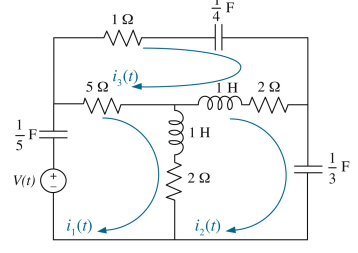
\includegraphics[width=\textwidth]{circuit}
		\caption{Circuit for Prelab 3}
		\label{fig:circuit}
	\end{figure}

	% Sit hierdie maar in as j dit kan reg kry maar vir nou sit ek net question 6 van lab se image in 
	\begin{equation}
		\label{eq:all}
		\begin{bmatrix}
		    \frac{s^2+7s+2}{s}	&	-s-2	&	-5\\
		    -s-2      			& 	\frac{2s^2+4s+3}{s}  & 	-s-2\\
		    -5      			& 	-s-2  & 	\frac{s^2+8s+4}{s}\\
		\end{bmatrix}
	\end{equation}

	\noindent Three additional matrices were constructed from the one in equation \ref{eq:all}, which will be used to derive the equations for the currents. They are shown respectively by equation \ref{eq:I1}, equation \ref{eq:I2} and equation \ref{eq:I3}. 

	\begin{equation}
		\label{eq:I1}
		I_{1 \text{num}}(s) =
		\begin{bmatrix}
		    V(s)	&	-s-2	&	-5\\
		    0    & 	\frac{2s^2+4s+3}{s}  & 	-s-2\\
		    0    & 	-s-2  & 	\frac{s^2+8s+4}{s}\\
		\end{bmatrix}
	\end{equation}

	\begin{equation}
		\label{eq:I2}
		I_{2 \text{num}}(s) =
		\begin{bmatrix}
		    \frac{s^2+7s+2}{s}	&	V(s)	&	-5\\
		    -s-2      			& 	0  & 	-s-2\\
		    -5      			& 	0  & 	\frac{s^2+8s+4}{s}\\
		\end{bmatrix}
	\end{equation}

	\begin{equation}
		\label{eq:I3}
		I_{3 \text{num}}(s) =
		\begin{bmatrix}
		    \frac{s^2+7s+2}{s}	&	-s-2	&	V(s)\\
		    -s-2      			& 	\frac{2s^2+4s+3}{s}  & 	0\\
		    -5      			& 	-s-2  & 	0\\
		\end{bmatrix}
	\end{equation}

	% \begin{figure}[H]
	% 	\centering
	% 	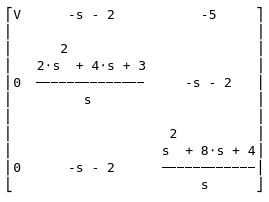
\includegraphics[width=\textwidth]{pre_lab_question_3_a1}
	% 	\caption{Matrix obtained for mesh current 1 - Matrix A1}
	% 	\label{fig:pre_lab_question_3_a1}
	% \end{figure}

	% \begin{figure}[H]
	% 	\centering
	% 	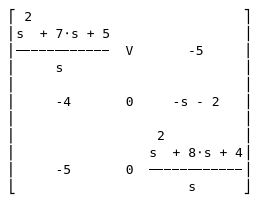
\includegraphics[width=\textwidth]{pre_lab_question_3_a2}
	% 	\caption{Matrix obtained for mesh current 2 - Matrix A2}
	% 	\label{fig:pre_lab_question_3_a2}
	% \end{figure}

	% \begin{figure}[H]
	% 	\centering
	% 	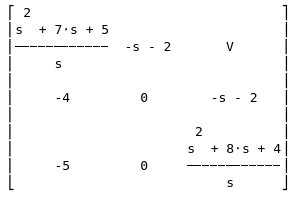
\includegraphics[width=\textwidth]{pre_lab_question_3_a3}
	% 	\caption{Matrix obtained mesh current 3 - Matrix A3}
	% 	\label{fig:pre_lab_question_3_a3}
	% \end{figure}

	\noindent The determinant of the original matrix A (equation \ref{eq:all}) is:\\
	\texttt{$s^3+12s^2+26s+153+\frac{380}{s}+\frac{284}{s^2}+\frac{60}{s^3}$}\\
	The determinant of the matrix $I_{1 \text{num}}(s)$ (equation \ref{eq:I1}) is:\\
	\texttt{$V(s)s^2+16V(s)s+39V(s)+\frac{40V(s)}{s}+\frac{12V(s)}{s^2}$}\\
	The determinant of the matrix $I_{2 \text{num}}(s)$ (equation \ref{eq:I2}) is:\\
	\texttt{$9Vs+42V+\frac{16V}{s}$}\\
	The determinant of the matrix $I_{1 \text{num}}(s)$ (equation \ref{eq:I3}) is:\\
	\texttt{$-9s^2-60s-100-\frac{32}{s}$}\\


	\noindent Now using Cramer's rule and the determinants of the original matrix, and those of the respective mesh current matrices, the mesh currents were found to be and are shown in the following equations:

	\begin{equation}
		\label{eq:I1_final}
		I_1(s) = \frac{s^2 + 16s + 39 + \frac{40}{s} + \frac{12}{s^2}}{s^3 + 14s^2 + 26s + 153 + \frac{380}{s} + \frac{284}{s^2} + \frac{60}{s^3}}V(s)
	\end{equation}

	\begin{equation}
		\label{eq:I2_final}
		I_2(s) = \frac{9s + 42 + \frac{16}{s}}{s^3 + 14s^2 + 26s + 153 + \frac{380}{s} + \frac{284}{s^2} + \frac{60}{s^3}}V(s)
	\end{equation}

	\begin{equation}
		\label{eq:I3_final}
		I_3(s) = \frac{9s^ - 60s - 100 - \frac{32}{s}}{s^3 + 14s^2 + 26s + 153 + \frac{380}{s} + \frac{284}{s^2} + \frac{60}{s^3}}V(s)
	\end{equation}

	% \begin{figure}[H]
	% 	\centering
	% 	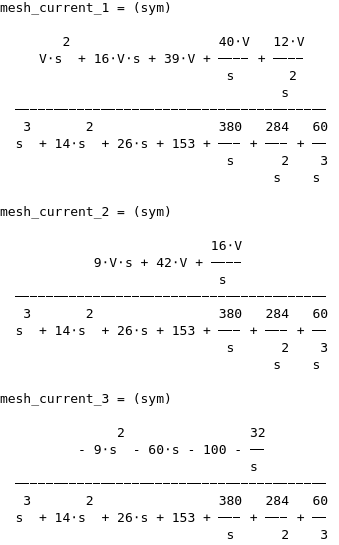
\includegraphics[width=\textwidth]{mesh_currents}
	% 	\caption{Mesh currents}
	% 	\label{fig:pre_lab_question_3_a3}
	% \end{figure}

	\noindent It is instructive to note that, without an expression for $V(s)$, we cannot explicitly find the mesh currents in the circuit, but we can implicitly solve them with the equations
	\[
		i_1(t) = \mathcal{L}^{-1}[I_1(s)] \quad i_2(t) = \mathcal{L}^{-1}[I_2(s)] \quad i_3(t) = \mathcal{L}^{-1}[I_3(s)]
	\]

	\newpage
	\section{Lab} % (fold)
	\subsection{Question 1}
	By first declaring a symbolic variable \texttt{t} and defining the function a symbolic function was returned\\


	\texttt{syms t;}\par
  	\texttt{f = 0.0075 - 0.0072 .* exp(-8 .* t) + 0.00034 .* exp(-2.5 .* t) .* cos(22 .* t) + 0.087 .* exp(-2.5 .*t ) .* sin(22 .* t);}\\

  	The results printed to the screen are shown by Figure \ref{fig:question_1}:\\

  	\begin{figure}[H]
		\centering
		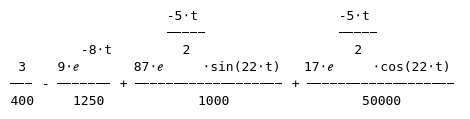
\includegraphics[width=\textwidth]{question_1}
		\caption{Results for Lab Question 1}
		\label{fig:question_1}
	\end{figure}

	\subsection*{Question 2}
	A symbolic representation of the transfer function (both in factored and simplified form) given in Prelab 2 resulted by executing the following commands:\\

	\texttt{syms s;}\\
    \texttt{numerator = 2*(s+3)*(s+5)*(s+7)}\\
    \texttt{denominator = s*(s+8)*(s\^{}2 +10*s +100)}\\
    \texttt{F = numerator/denominator}\\
    \texttt{expanded = expand(F);}\\
    \texttt{simplified = simplify(F);}\\


    Figure \ref{fig:question_2} shows these results:\\

    \begin{figure}[H]
		\centering
		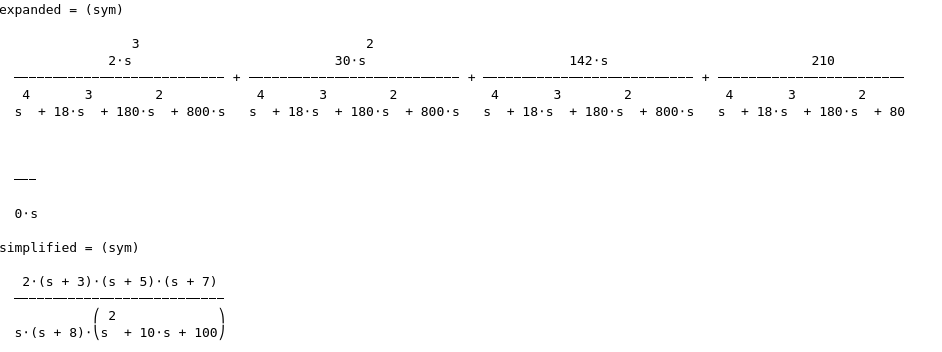
\includegraphics[width=\textwidth]{question_2}
		\caption{Results for Lab Question 2}
		\label{fig:question_2}
	\end{figure}

	\subsection{Question 3}
	The laplace transform of the function \texttt{f(t)} from Prelab 1 was calculated by running the code that follows in Octave:\\
	
	\texttt{syms t;}\par
  	\texttt{f = 0.0075 - 0.0072 .* exp(-8 .* t) + 0.00034 .* exp(-2.5 .* t) .* cos(22 .* t) + 0.087 .* exp(-2.5 .*t ) .* sin(22 .* t);}\par
  	\texttt{F = laplace(f);}\par
  	\texttt{expanded = expand(F);}\par
  	\texttt{simplified = simplify(F);}\\

  	The results are shown in Figure \ref{fig:question_3}:\\

  	\begin{figure}[H]
		\centering
		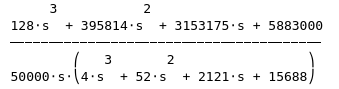
\includegraphics[width=\textwidth]{question_3}
		\caption{Results for Lab Question 3}
		\label{fig:question_3}
	\end{figure}


	\subsection{Question 4}
	The code shown below gave the inverse Laplace transform of the function given in Prelab 2:\\

	\texttt{syms s;}\par
  	\texttt{numerator = 2*(s+3)*(s+5)*(s+7);}\par
  	\texttt{denominator = s*(s+8)*(s\^2 +10*s +100);}\par
  	\texttt{F = numerator/denominator;}\par
  	\texttt{inverse = ilaplace(F);}\\

  	This gave the results depicted in Figure \ref{fig:question_4} \\


	\begin{figure}[H]
		\centering
		
\includegraphics[width=\textwidth]{question_4}
		\caption{Results for Lab Question 4}
		\label{fig:question_4}
	\end{figure}


	\subsection{Question 5}

	\subsection{Question 6}
	Considering the circuit from Prelab 3, a matrix was found using mesh analysis. The terms that were obtained were entered into Octave according to the following code:\\

	\texttt{syms s V;} \par
	\texttt{t1 = (s\^{}2 + 7*s + 5)/s;}\par
	\texttt{t2 = -s-2;}\par
	\texttt{t3 = -5;}\par
	\texttt{t4 = -2-2;}\par
	\texttt{t5 = (2*s\^{}2 + 4*s + 3)/s;}\par
	\texttt{t6 = -s-2;}\par
	\texttt{t7 = -5;}\par
	\texttt{t8 = -s-2;}\par
	\texttt{t9 = (s\^{}2+8*s+4)/s;}\\

	\texttt{matrix = [t1,t2,t3;t4,t5,t6;t7,t8,t9];}\\

	The matrix obtained is shown in Figure \ref{fig:question_6}:\\
	
	\begin{figure}[H]
		\centering
		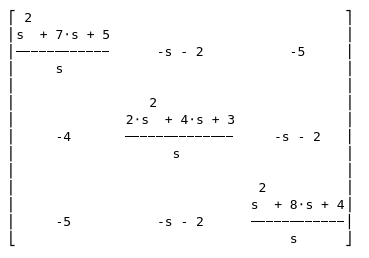
\includegraphics[width=\textwidth]{question_6}
		\caption{Results for Lab Question 6}
		\label{fig:question_6}
	\end{figure}

	In order to make use of Cramer's  rule to find the mesh currents $I_1$, $I_2$ and $I_3$ we had to construct 3 additional matrices from the matrix shown in Figure \ref{fig:question_6} and find their determinants as well as that of the original matrix. We executed the following code to yield us these results:\\

	\texttt{determinant\_matrix = expand(det(matrix));}\par

	
  	\texttt{matrix\_a1 = [V, t2, t3;0, t5, t6;0, t8, t9];}\par
  	\texttt{matrix\_a2 = [t1,V,t3;t4,0,t6;t7,0,t9];}\par
  	\texttt{matrix\_a3 = [t1,t2,V;t4,0,t6;t7,0,t9];}\par

  	\texttt{determinant\_matrix\_a1 = expand(det(matrix\_a1));}\par
  	\texttt{determinant\_matrix\_a2 = expand(det(matrix\_a2));}\par
  	\texttt{determinant\_matrix\_a3 = expand(det(matrix\_a3));}\par

  	From the calculated determinants, Cramer's rule was used to find the mesh currents by running the following in Octave:\\

  	\texttt{mesh\_current\_1 =  determinant\_matrix\_a1/determinant\_matrix;}\par
	\texttt{mesh\_current\_2 =  determinant\_matrix\_a2/determinant\_matrix;}\par
	\texttt{mesh\_current\_3 =  determinant\_matrix\_a3/determinant\_matrix;}\par
	% section Lab (end)

	\section{Post Lab}
	The advantage to using the Symbolic Math Toolbox is that it allows the user of the package to see the expressions the way we are use to seeing them (as we would write them down on a piece of paper). Using this package allowed us to achieve exactly this. This would not have been possible to do using the native Ocatve functions to execute the Laplace transform and inverse Laplace transform operations in functions. 
\end{document}